%---------------
%╔═╗╔═╗╔╦╗╦ ╦╔═╗
%╚═╗║╣  ║ ║ ║╠═╝
%╚═╝╚═╝ ╩ ╚═╝╩  
%---------------

% language setup
\newcommand{\docLanguage}{ngerman}
%\newcommand{\docLanguage}{english}

% DOCUMENT SETUP
\documentclass[12pt, oneside, a4paper, \docLanguage]{report}
\usepackage[left=3cm, 
			right=2.5cm, 
			top=2.5cm, 
			bottom=2.5cm, 
			includehead, 
			includefoot]{geometry}

% line spacing
\usepackage{setspace}
\setstretch{1,25} % 15/12 --> 1.25

% encoding setup
% T1 font encoding for languages that use a latin alphabet
\usepackage[T1]{fontenc} 

% enhanced input encoding handling - utf8 for äÄüÜöÖß...
\usepackage[utf8]{inputenc}

%de­fines Adobe Times Ro­man as de­fault text font
\usepackage{mathptmx}
\usepackage{times} % needed for acronym package

%PDF linking package
\usepackage[hidelinks]{hyperref}


% Language Setup
\usepackage[\docLanguage]{babel}
% after babel - set chapter string
\AtBeginDocument{\renewcommand{\chaptername}{}}

% language specific bibliography style
\usepackage[numbers, square]{natbib}
%\setcitestyle{square,aysep={},yysep={;}}
\usepackage[fixlanguage]{babelbib}
\selectbiblanguage{\docLanguage}
% bliographystyle setup
% babel specific: babplain, babplai3, babalpha, babunsrt, bababbrv, bababbr3
\bibliographystyle{babunsrt}


% enumeration
\usepackage{enumitem}
% tabular extension tabularx
\usepackage{tabularx}

% math packages
\usepackage{amsmath}
\usepackage{nicefrac}
\usepackage{amsthm}
\usepackage{amsbsy}
\usepackage{amssymb}
\usepackage{amsfonts}
%\usepackage{MnSymbol}


%special characters
\usepackage{amssymb}
\usepackage{upgreek,textgreek}

% acronym package
\usepackage[printonlyused, footnote]{acronym}

% breakable text in \seqsplit{}
\usepackage{seqsplit}

% \textmu
\usepackage{textcomp}

% package provides a way to compile sections of a document using the same preamble as the main document
\usepackage{subfiles}

% driver-independent color extension - used by listings,tabularx
\usepackage[usenames,dvipsnames,table,xcdraw]{xcolor}

% -- SYNTAX HIGHLIGHTING --
\usepackage{listings}
%% bash command line Syntax Highlighting
\lstdefinestyle{BASH_CMD}{ 
  columns=fullflexible,            % copy pasteable listings
  language=bash,
  basicstyle=\small\sffamily,
  basicstyle   = \small \ttfamily,
  keywordstyle = [1]\small \ttfamily,
  keywordstyle = [2]\small \ttfamily,
  commentstyle = \small \ttfamily,
  numbers=none,
  captionpos=b, 
  breaklines=true,
  numberstyle=\tiny,
  numbersep=3pt,
  frame=tlrb,
  columns=fullflexible,
  backgroundcolor=\color{white!20},
  linewidth=\linewidth,
  literate=                        % replace in code
     {Ö}{{\"O}}1 
     {Ä}{{\"A}}1 
     {Ü}{{\"U}}1 
     {ß}{{\ss}}2 
     {ü}{{\"u}}1 
     {ä}{{\"a}}1 
     {ö}{{\"o}}1 
     {â}{{\^{a}}}1 
     {Â}{{\^{A}}}1 
     {ç}{{\c{c}}}1 
     {Ç}{{\c{C}}}1 
     {ğ}{{\u{g}}}1 
     {Ğ}{{\u{G}}}1 
     {ı}{{\i}}1 
     {İ}{{\.{I}}}1 
     {ş}{{\c{s}}}1 
     {Ş}{{\c{S}}}1 
}
 % adds style BASH_CMD
%% Matlab Syntax Highlighting
\colorlet{keyword}{blue!100!black!80}
\colorlet{STD}{Lavender}
\colorlet{comment}{green!90!black!90}
\definecolor{mygreen}{rgb}{0,0.6,0}
\definecolor{mygray}{rgb}{0.5,0.5,0.5}
\definecolor{mymauve}{rgb}{0.58,0,0.82}


\lstdefinestyle{BASH_SCRIPT}{ 
  language     = bash,
  basicstyle   = \footnotesize \ttfamily,
  keywordstyle = [1]\color{keyword}\bfseries,
  keywordstyle = [2]\color{STD}\bfseries,
  commentstyle = \color{mygreen}\itshape,
  backgroundcolor=\color{white},   % choose the background color; you must add \usepackage{color} 
  columns=fullflexible,            % copy pasteable listings
                                   % or \usepackage{xcolor}
  basicstyle=\footnotesize,        % the size of the fonts that are used for the code
  breakatwhitespace=false,         % sets if automatic breaks should only happen at whitespace
  breaklines=true,                 % sets automatic line breaking
  captionpos=b,                    % sets the caption-position to bottom
  extendedchars=true,              % lets you use non-ASCII characters; for 8-bits encodings only,
                                   % does not work with UTF-8
  frame=single,                    % adds a frame around the code
  keepspaces=true,                 % keeps spaces in text, useful for keeping indentation of code
                                   % (possibly needs columns=flexible)
  numbers=left,                    % where to put the line-numbers; possible values are 
                                   % (none, left, right)
  numbersep=5pt,                   % how far the line-numbers are from the code
  numberstyle=\tiny\color{mygray}, % the style that is used for the line-numbers
  rulecolor=\color{black},         % if not set, the frame-color may be changed on line-breaks
                                   % within not-black text (e.g. comments (green here))
  showspaces=false,                % show spaces everywhere adding particular underscores; it
  	                               % overrides 'showstringspaces'
  showstringspaces=false,          % underline spaces within strings only
  showtabs=false,                  % show tabs within strings adding particular underscores
  stepnumber=1,                    % the step between two line-numbers. If it's 1, each line 
                                   % will be numbered
  stringstyle=\color{mymauve},     % string literal style
  tabsize=2,                       % sets default tabsize to 2 spaces
  title=\lstname,                  % set title name
  literate=                        % replace in code
     {Ö}{{\"O}}1 
     {Ä}{{\"A}}1 
     {Ü}{{\"U}}1 
     {ß}{{\ss}}2 
     {ü}{{\"u}}1 
     {ä}{{\"a}}1 
     {ö}{{\"o}}1 
     {â}{{\^{a}}}1 
     {Â}{{\^{A}}}1 
     {ç}{{\c{c}}}1 
     {Ç}{{\c{C}}}1 
     {ğ}{{\u{g}}}1 
     {Ğ}{{\u{G}}}1 
     {ı}{{\i}}1 
     {İ}{{\.{I}}}1 
     {ş}{{\c{s}}}1 
     {Ş}{{\c{S}}}1 
} % adds style BASH_SCRIPT
% Matlab Syntax Highlighting
\colorlet{keyword}{blue!100!black!80}
\colorlet{STD}{red}
\colorlet{comment}{green!90!black!90}
\definecolor{mygreen}{rgb}{0,0.6,0}
\definecolor{mygray}{rgb}{0.5,0.5,0.5}
\definecolor{mymauve}{rgb}{0.58,0,0.82}


\lstdefinestyle{LATEX}{ 
  language     = [LaTeX]{TeX},
  basicstyle   = \footnotesize \ttfamily,
  keywordstyle = [1]\color{keyword}\bfseries,
  keywordstyle = [2]\color{comment}\bfseries,
  commentstyle = \color{mygray}\itshape,
  %backgroundcolor=\color{white},   % choose the background color; you must add \usepackage{color} 
                                   % or \usepackage{xcolor}
  basicstyle=\footnotesize,        		   % the size of the fonts that are used for the code
  breakatwhitespace=false,         % sets if automatic breaks should only happen at whitespace
  columns=fullflexible,            % copy pasteable listings
  breaklines=true,                 % sets automatic line breaking
  captionpos=c,                    % sets the caption-position to bottom
  extendedchars=true,              % lets you use non-ASCII characters; for 8-bits encodings only,
                                   % does not work with UTF-8
  frame=single,                    % adds a frame around the code
  keepspaces=true,                 % keeps spaces in text, useful for keeping indentation of code
                                   % (possibly needs columns=flexible)
  numbers=left,                    % where to put the line-numbers; possible values are 
                                   % (none, left, right)
  numbersep=4pt,                   % how far the line-numbers are from the code
  numberstyle=\tiny\color{mygray}, % the style that is used for the line-numbers
  rulecolor=\color{black},         % if not set, the frame-color may be changed on line-breaks
                                   % within not-black text (e.g. comments (green here))
  showspaces=false,                % show spaces everywhere adding particular underscores; it
  	                               % overrides 'showstringspaces'
  showstringspaces=false,          % underline spaces within strings only
  showtabs=false,                  % show tabs within strings adding particular underscores
  stepnumber=1,                    % the step between two line-numbers. If it's 1, each line 
                                   % will be numbered
  stringstyle=\color{mymauve},     % string literal style
  tabsize=2,                       % sets default tabsize to 2 spaces
  title=\lstname,                  % set title name
  literate=                        % replace in code
     {Ö}{{\"O}}1 
     {Ä}{{\"A}}1 
     {Ü}{{\"U}}1 
     {ß}{{\ss}}2 
     {ü}{{\"u}}1 
     {ä}{{\"a}}1 
     {ö}{{\"o}}1 
     {â}{{\^{a}}}1 
     {Â}{{\^{A}}}1 
     {ç}{{\c{c}}}1 
     {Ç}{{\c{C}}}1 
     {ğ}{{\u{g}}}1 
     {Ğ}{{\u{G}}}1 
     {ı}{{\i}}1 
     {İ}{{\.{I}}}1 
     {ş}{{\c{s}}}1 
     {Ş}{{\c{S}}}1 
} % adds style LATEX
%% Matlab Syntax Highlighting
\colorlet{keyword}{blue!100!black!80}
\colorlet{STD}{Lavender}
\colorlet{comment}{green!90!black!90}
\definecolor{mygreen}{rgb}{0,0.6,0}
\definecolor{mygray}{rgb}{0.5,0.5,0.5}
\definecolor{mymauve}{rgb}{0.58,0,0.82}


\lstdefinestyle{MATLAB}{ 
  language     = Matlab,
  basicstyle   = \footnotesize \ttfamily,
  keywordstyle = [1]\color{keyword}\bfseries,
  keywordstyle = [2]\color{STD}\bfseries,
  commentstyle = \color{mygreen}\itshape,
  backgroundcolor=\color{white},   % choose the background color; you must add \usepackage{color} 
                                   % or \usepackage{xcolor}
  basicstyle=\footnotesize,        % the size of the fonts that are used for the code
  breakatwhitespace=false,         % sets if automatic breaks should only happen at whitespace
  columns=fullflexible,            % copy pasteable listings
  breaklines=false,                % sets automatic line breaking
  captionpos=c,                    % sets the caption-position to bottom
  extendedchars=true,              % lets you use non-ASCII characters; for 8-bits encodings only,
                                   % does not work with UTF-8
  frame=single,                    % adds a frame around the code
  keepspaces=true,                 % keeps spaces in text, useful for keeping indentation of code
                                   % (possibly needs columns=flexible)
  numbers=left,                    % where to put the line-numbers; possible values are 
                                   % (none, left, right)
  numbersep=5pt,                   % how far the line-numbers are from the code
  numberstyle=\tiny\color{mygray}, % the style that is used for the line-numbers
  rulecolor=\color{black},         % if not set, the frame-color may be changed on line-breaks
                                   % within not-black text (e.g. comments (green here))
  showspaces=false,                % show spaces everywhere adding particular underscores; it
  	                               % overrides 'showstringspaces'
  showstringspaces=false,          % underline spaces within strings only
  showtabs=false,                  % show tabs within strings adding particular underscores
  stepnumber=1,                    % the step between two line-numbers. If it's 1, each line 
                                   % will be numbered
  stringstyle=\color{mymauve},     % string literal style
  tabsize=2,                       % sets default tabsize to 2 spaces
  title=\lstname,                  % set title name
  literate=                        % replace in code
     {Ö}{{\"O}}1 
     {Ä}{{\"A}}1 
     {Ü}{{\"U}}1 
     {ß}{{\ss}}2 
     {ü}{{\"u}}1 
     {ä}{{\"a}}1 
     {ö}{{\"o}}1 
     {â}{{\^{a}}}1 
     {Â}{{\^{A}}}1 
     {ç}{{\c{c}}}1 
     {Ç}{{\c{C}}}1 
     {ğ}{{\u{g}}}1 
     {Ğ}{{\u{G}}}1 
     {ı}{{\i}}1 
     {İ}{{\.{I}}}1 
     {ş}{{\c{s}}}1 
     {Ş}{{\c{S}}}1 
} % adds style MATLAB
% Matlab Syntax Highlighting
\colorlet{keyword}{blue!100!black!80}
\colorlet{STD}{Lavender}
\colorlet{comment}{green!90!black!90}
\definecolor{mygreen}{rgb}{0,0.6,0}
\definecolor{mygray}{rgb}{0.5,0.5,0.5}
\definecolor{mymauve}{rgb}{0.58,0,0.82}


\lstdefinestyle{PYTHON}{ 
  language     = Python,
  basicstyle   = \footnotesize \ttfamily,
  keywordstyle = [1]\color{keyword}\bfseries,
  keywordstyle = [2]\color{STD}\bfseries,
  commentstyle = \color{mygreen}\itshape,
  backgroundcolor=\color{white},   % choose the background color; you must add \usepackage{color} 
                                   % or \usepackage{xcolor}
  basicstyle=\footnotesize,        % the size of the fonts that are used for the code
  columns=fullflexible,            % copy pasteable listings
  breakatwhitespace=false,         % sets if automatic breaks should only happen at whitespace
  breaklines=false,                % sets automatic line breaking
  captionpos=c,                    % sets the caption-position to bottom
  extendedchars=true,              % lets you use non-ASCII characters; for 8-bits encodings only,
                                   % does not work with UTF-8
  frame=single,                    % adds a frame around the code
  keepspaces=true,                 % keeps spaces in text, useful for keeping indentation of code
                                   % (possibly needs columns=flexible)
  numbers=left,                    % where to put the line-numbers; possible values are 
                                   % (none, left, right)
  numbersep=5pt,                   % how far the line-numbers are from the code
  numberstyle=\tiny\color{mygray}, % the style that is used for the line-numbers
  rulecolor=\color{black},         % if not set, the frame-color may be changed on line-breaks
                                   % within not-black text (e.g. comments (green here))
  showspaces=false,                % show spaces everywhere adding particular underscores; it
  	                               % overrides 'showstringspaces'
  showstringspaces=false,          % underline spaces within strings only
  showtabs=false,                  % show tabs within strings adding particular underscores
  stepnumber=1,                    % the step between two line-numbers. If it's 1, each line 
                                   % will be numbered
  stringstyle=\color{mymauve},     % string literal style
  tabsize=2,                       % sets default tabsize to 2 spaces
  title=\lstname,                  % set title name
  literate=                        % replace in code
     {Ö}{{\"O}}1 
     {Ä}{{\"A}}1 
     {Ü}{{\"U}}1 
     {ß}{{\ss}}2 
     {ü}{{\"u}}1 
     {ä}{{\"a}}1 
     {ö}{{\"o}}1 
     {â}{{\^{a}}}1 
     {Â}{{\^{A}}}1 
     {ç}{{\c{c}}}1 
     {Ç}{{\c{C}}}1 
     {ğ}{{\u{g}}}1 
     {Ğ}{{\u{G}}}1 
     {ı}{{\i}}1 
     {İ}{{\.{I}}}1 
     {ş}{{\c{s}}}1 
     {Ş}{{\c{S}}}1 
} % adds style PYTHON
%% Matlab Syntax Highlighting
\colorlet{keyword}{blue!100!black!80}
\colorlet{STD}{Lavender}
\colorlet{comment}{green!90!black!90}
\definecolor{mygreen}{rgb}{0,0.6,0}
\definecolor{mygray}{rgb}{0.5,0.5,0.5}
\definecolor{mymauve}{rgb}{0.58,0,0.82}


\lstdefinestyle{CPP}{ 
  language     = C++,
  basicstyle   = \footnotesize \ttfamily,
  keywordstyle = [1]\color{keyword}\bfseries,
  keywordstyle = [2]\color{STD}\bfseries,
  commentstyle = \color{mygreen}\itshape,
  backgroundcolor=\color{white},   % choose the background color; you must add \usepackage{color} 
                                   % or \usepackage{xcolor}
  columns=fullflexible,            % copy pasteable listings
  basicstyle=\footnotesize,        % the size of the fonts that are used for the code
  breakatwhitespace=false,         % sets if automatic breaks should only happen at whitespace
  breaklines=false,                % sets automatic line breaking
  captionpos=c,                    % sets the caption-position to bottom
  extendedchars=true,              % lets you use non-ASCII characters; for 8-bits encodings only,
                                   % does not work with UTF-8
  frame=single,                    % adds a frame around the code
  keepspaces=true,                 % keeps spaces in text, useful for keeping indentation of code
                                   % (possibly needs columns=flexible)
  numbers=left,                    % where to put the line-numbers; possible values are 
                                   % (none, left, right)
  numbersep=5pt,                   % how far the line-numbers are from the code
  numberstyle=\tiny\color{mygray}, % the style that is used for the line-numbers
  rulecolor=\color{black},         % if not set, the frame-color may be changed on line-breaks
                                   % within not-black text (e.g. comments (green here))
  showspaces=false,                % show spaces everywhere adding particular underscores; it
  	                               % overrides 'showstringspaces'
  showstringspaces=false,          % underline spaces within strings only
  showtabs=false,                  % show tabs within strings adding particular underscores
  stepnumber=1,                    % the step between two line-numbers. If it's 1, each line 
                                   % will be numbered
  stringstyle=\color{mymauve},     % string literal style
  tabsize=2,                       % sets default tabsize to 2 spaces
  title=\lstname,                  % set title name
  literate=                        % replace in code
     {Ö}{{\"O}}1 
     {Ä}{{\"A}}1 
     {Ü}{{\"U}}1 
     {ß}{{\ss}}2 
     {ü}{{\"u}}1 
     {ä}{{\"a}}1 
     {ö}{{\"o}}1 
     {â}{{\^{a}}}1 
     {Â}{{\^{A}}}1 
     {ç}{{\c{c}}}1 
     {Ç}{{\c{C}}}1 
     {ğ}{{\u{g}}}1 
     {Ğ}{{\u{G}}}1 
     {ı}{{\i}}1 
     {İ}{{\.{I}}}1 
     {ş}{{\c{s}}}1 
     {Ş}{{\c{S}}}1 
} % adds style CPP
%% Matlab Syntax Highlighting
\colorlet{keyword}{blue!100!black!80}
\colorlet{STD}{Lavender}
\colorlet{comment}{green!90!black!90}
\definecolor{mygreen}{rgb}{0,0.6,0}
\definecolor{mygray}{rgb}{0.5,0.5,0.5}
\definecolor{mymauve}{rgb}{0.58,0,0.82}


\lstdefinestyle{C}{ 
  language     = C,
  basicstyle   = \footnotesize \ttfamily,
  keywordstyle = [1]\color{keyword}\bfseries,
  keywordstyle = [2]\color{STD}\bfseries,
  commentstyle = \color{mygreen}\itshape,
  backgroundcolor=\color{white},   % choose the background color; you must add \usepackage{color} 
  columns=fullflexible,            % copy pasteable listings
                                   % or \usepackage{xcolor}
  basicstyle=\footnotesize,        % the size of the fonts that are used for the code
  breakatwhitespace=false,         % sets if automatic breaks should only happen at whitespace
  breaklines=false,                % sets automatic line breaking
  captionpos=c,                    % sets the caption-position to bottom
  extendedchars=true,              % lets you use non-ASCII characters; for 8-bits encodings only,
                                   % does not work with UTF-8
  frame=single,                    % adds a frame around the code
  keepspaces=true,                 % keeps spaces in text, useful for keeping indentation of code
                                   % (possibly needs columns=flexible)
  numbers=left,                    % where to put the line-numbers; possible values are 
                                   % (none, left, right)
  numbersep=5pt,                   % how far the line-numbers are from the code
  numberstyle=\tiny\color{mygray}, % the style that is used for the line-numbers
  rulecolor=\color{black},         % if not set, the frame-color may be changed on line-breaks
                                   % within not-black text (e.g. comments (green here))
  showspaces=false,                % show spaces everywhere adding particular underscores; it
  	                               % overrides 'showstringspaces'
  showstringspaces=false,          % underline spaces within strings only
  showtabs=false,                  % show tabs within strings adding particular underscores
  stepnumber=1,                    % the step between two line-numbers. If it's 1, each line 
                                   % will be numbered
  stringstyle=\color{mymauve},     % string literal style
  tabsize=2,                       % sets default tabsize to 2 spaces
  title=\lstname,                  % set title name
  literate=                        % replace in code
     {Ö}{{\"O}}1 
     {Ä}{{\"A}}1 
     {Ü}{{\"U}}1 
     {ß}{{\ss}}2 
     {ü}{{\"u}}1 
     {ä}{{\"a}}1 
     {ö}{{\"o}}1 
     {â}{{\^{a}}}1 
     {Â}{{\^{A}}}1 
     {ç}{{\c{c}}}1 
     {Ç}{{\c{C}}}1 
     {ğ}{{\u{g}}}1 
     {Ğ}{{\u{G}}}1 
     {ı}{{\i}}1 
     {İ}{{\.{I}}}1 
     {ş}{{\c{s}}}1 
     {Ş}{{\c{S}}}1 
} % adds style C
%% JSON Syntax Highlighting
\colorlet{keyword}{blue!100!black!80}
\colorlet{STD}{Lavender}
\colorlet{comment}{green!90!black!90}
\definecolor{mygreen}{rgb}{0,0.6,0}
\definecolor{mygray}{rgb}{0.5,0.5,0.5}
\definecolor{mymauve}{rgb}{0.58,0,0.82}

\newcommand\JSONnumbervaluestyle{\color{blue}}
\newcommand\JSONstringvaluestyle{\color{red}}

\newif\ifcolonfoundonthisline

\makeatletter

\lstdefinelanguage{json}
{
  showstringspaces    = false,
  keywords            = {false,true},
  alsoletter          = 0123456789.,
  morestring          = [s]{"}{"},
  morestring          = [s]{'}{'},
  stringstyle         = \ifcolonfoundonthisline\JSONstringvaluestyle\fi,
  MoreSelectCharTable =%
    \lst@DefSaveDef{`:}\colon@json{\processColon@json},
  basicstyle          = \ttfamily,
  keywordstyle        = \ttfamily\bfseries,
}

% flip the switch if a colon is found in Pmode
\newcommand\processColon@json{
  \colon@json%
  \ifnum\lst@mode=\lst@Pmode%
    \global\colonfoundonthislinetrue%
  \fi
}

\lst@AddToHook{Output}{%
  \ifcolonfoundonthisline%
    \ifnum\lst@mode=\lst@Pmode%
      \def\lst@thestyle{\JSONnumbervaluestyle}%
    \fi
  \fi
  %override by keyword style if a keyword is detected!
  \lsthk@DetectKeywords% 
}

% reset the switch at the end of line
\lst@AddToHook{EOL}%
  {\global\colonfoundonthislinefalse}

\makeatother



\lstdefinestyle{JSON}{ 
  language     = json,
  basicstyle   = \footnotesize \ttfamily,
  keywordstyle = [1]\color{keyword}\bfseries,
  keywordstyle = [2]\color{STD}\bfseries,
  commentstyle = \color{mygreen}\itshape,
  backgroundcolor=\color{white},   % choose the background color; you must add \usepackage{color} 
                                   % or \usepackage{xcolor}
  basicstyle=\footnotesize,        % the size of the fonts that are used for the code
  columns=fullflexible,            % copy pasteable listings
  breakatwhitespace=false,         % sets if automatic breaks should only happen at whitespace
  breaklines=false,                % sets automatic line breaking
  captionpos=c,                    % sets the caption-position to bottom
  extendedchars=true,              % lets you use non-ASCII characters; for 8-bits encodings only,
                                   % does not work with UTF-8
  frame=single,                    % adds a frame around the code
  keepspaces=true,                 % keeps spaces in text, useful for keeping indentation of code
                                   % (possibly needs columns=flexible)
  numbers=left,                    % where to put the line-numbers; possible values are 
                                   % (none, left, right)
  numbersep=5pt,                   % how far the line-numbers are from the code
  numberstyle=\tiny\color{mygray}, % the style that is used for the line-numbers
  rulecolor=\color{black},         % if not set, the frame-color may be changed on line-breaks
                                   % within not-black text (e.g. comments (green here))
  showspaces=false,                % show spaces everywhere adding particular underscores; it
  	                               % overrides 'showstringspaces'
  showstringspaces=false,          % underline spaces within strings only
  showtabs=false,                  % show tabs within strings adding particular underscores
  stepnumber=1,                    % the step between two line-numbers. If it's 1, each line 
                                   % will be numbered
  stringstyle=\color{mymauve},     % string literal style
  tabsize=2,                       % sets default tabsize to 2 spaces
  title=\lstname,                  % set title name
  literate=                        % replace in code
     {Ö}{{\"O}}1 
     {Ä}{{\"A}}1 
     {Ü}{{\"U}}1 
     {ß}{{\ss}}2 
     {ü}{{\"u}}1 
     {ä}{{\"a}}1 
     {ö}{{\"o}}1 
     {â}{{\^{a}}}1 
     {Â}{{\^{A}}}1 
     {ç}{{\c{c}}}1 
     {Ç}{{\c{C}}}1 
     {ğ}{{\u{g}}}1 
     {Ğ}{{\u{G}}}1 
     {ı}{{\i}}1 
     {İ}{{\.{I}}}1 
     {ş}{{\c{s}}}1 
     {Ş}{{\c{S}}}1 
} % adds style JSON

% HEADLINE CFG
\usepackage{fancyhdr} % Headers and footers
\usepackage{lastpage}
\usepackage{ifthen}
\setlength{\headheight}{1.5cm}
%\pagestyle{fancy} % All pages have headers and footers
% override plain page style for \part, \chapter or 
% \maketitle, which implicit specifies plain page style
\fancypagestyle{plain} 
{
	\fancyhead[L]{}
	\fancyhead[C]{}
	\fancyhead[R]{}
	\fancyfoot[L]{}
	\fancyfoot[C]{\thepage}
	\fancyfoot[R]{}
}
% set list pagestyle
\fancypagestyle{preface} 
{
	\fancyhead[L]{}
	\fancyhead[C]{}
	\fancyhead[R]{}
	\fancyfoot[L]{}
	\fancyfoot[C]{\thepage}
	\fancyfoot[R]{}
}
% set default pagestyle
\fancypagestyle{default} 
{
	\fancyhead{} % Blank out the default header
	\fancyfoot{} % Blank out the default footer
	\fancyhead[L]{}
	\fancyhead[C]{}
	\fancyhead[R]{}
	\fancyfoot[L]{}
	\fancyfoot[C]{\thepage}
	\fancyfoot[R]{}
}
%\fancypagestyle{default} 
{
\fancyhead[L]{\ifthenelse{\isodd{\value{page}}}{\arabic{chapter} \rightmark}{}}
\fancyhead[R]{\thepage}
}

\renewcommand{\chaptermark}[1]{\markright{#1}{}}
\renewcommand{\sectionmark}[1]{\markright{#1}{}}
\renewcommand{\headrulewidth}{0pt}
\renewcommand{\footrulewidth}{0pt}

% PICTURE CFG 
\usepackage{verbatim}
\usepackage{graphicx}
\usepackage{subfig}

\usepackage{epstopdf}
\usepackage{caption}
\usepackage[list=true,listformat=simple]{subcaption}
% floating prevention packages
\usepackage{float}    % used with [H] positioning parameter
\usepackage{placeins} % \FloatBarrier 
% tikz packages
\usepackage{tikz}
\usepackage{standalone}
\usepackage{pgfplots}


% include only specified tex files - uncommend here
\includeonly{preface/cover,
             preface/abstract,
             preface/tableofcontents,
             preface/listoffigures,
             preface/listoftables,
             preface/lstlistoflistings,
             appendix/bibliography}

%-------------------
%╔═╗╔╦╗╦═╗╦╔╗╔╔═╗╔═╗
%╚═╗ ║ ╠╦╝║║║║║ ╦╚═╗
%╚═╝ ╩ ╩╚═╩╝╚╝╚═╝╚═╝
%-------------------
\newcommand{\strLecture}{Signale, Systeme und Sensoren}
\newcommand{\strDate}{\today}
\newcommand{\strAuthorA}{T. Schoch}
\newcommand{\strAuthorB}{L. Stratmann}
%\newcommand{\strAuthorC}{C. Author}
\newcommand{\strAuthorAEmail}{tobias.schoch@htwg-konstanz.de}
\newcommand{\strAuthorBEmail}{luca.stratmann@htwg-konstanz.de}
%\newcommand{\strAuthorCEmail}{cauthor@htwg-konstanz.de}
% Versuchsbeschreibung 
\newcommand{\strTopic}{Kalibrierung von digitalen Kameras}
\newcommand{\strAbstract}{In dem Versuch haben wir einen Entfernungsmesser dazu verwendet, um die bereits in der Vorlesung behandelten Vorgehensweisen zum Thema Kalibrierung, Fehlerbehandlung und Fehlerrechnung anzuwenden.
Der Distanzsensor der Marke "Sharp" benutzt für das Triangulationsprinzip Infrarot-LEDS mit einer Linse. Diese geben Lichtstrahlen von sich, um dann wiederrum reflektiert zu werden und durch die zweite Linse zu gelangen.
Je nachdem wo der Lichtstrahl auftrifft, wandelt der Signalprozessor die Leitfähigkeit in eine Spannung um.
Da das Ausgangssignal anti-proportional ist, wird mit der zunehmenden Entfernung das Ausgangssignal kleiner.
Die Entfernungen liegen zwischen 10cm und 70cm. Durch ein Oszillsokop können wir den Spannungsverlauf des Abstandssensors überprüfen.
 }
% hyperref customization
\hypersetup{
	pdftitle     = {\strTopic}, % title
	pdfsubject   = {\strLecture}, % subject of the document
	pdfauthor    = {\strAuthorA, \strAuthorB}, % author
	pdfkeywords  = {}, % list of keywords
	pdfcreator   = {}, % creator of the document
	pdfproducer  = {}, % producer of the document
	colorlinks   = false, % false: boxed links; true: colored links
	linkcolor    = red, % color of internal links (change box color with linkbordercolor)
    citecolor    = green, % color of links to bibliography
    filecolor    = magenta, % color of file links
    urlcolor     = cyan, % color of external links
	%bookmarks    = true, % show bookmarks bar?
	unicode	     = true, % non-Latin characters in Acrobat’s bookmarks
	pdftoolbar   = true, % show Acrobat’s toolbar?
	pdfmenubar   = true, % show Acrobat’s menu?
    pdffitwindow = false, % window fit to page when opened
	pdfnewwindow = true % links in new PDF window
}

%-----------------------------------------
% ╔╗ ╔═╗╔═╗╦╔╗╔  ╔╦╗╔═╗╔═╗╦ ╦╔╦╗╔═╗╔╗╔╔╦╗ 
% ╠╩╗║╣ ║ ╦║║║║   ║║║ ║║  ║ ║║║║║╣ ║║║ ║  
% ╚═╝╚═╝╚═╝╩╝╚╝  ═╩╝╚═╝╚═╝╚═╝╩ ╩╚═╝╝╚╝ ╩  
%-----------------------------------------

\begin{document}
\pagenumbering{Roman} 

\setcounter{section}{0}

\begin{titlepage}

\vspace*{-3.5cm}

\begin{flushleft}
\hspace*{-1cm} 
\includegraphics[width=15.7cm]{preface/htwg-logo.png}
\end{flushleft}

\vspace{1cm}

\begin{center}
	\large{
		\textbf{\strLecture} \\[2cm]
	}
	\Huge{
		\textbf{\strTopic} \\[2cm]
	}
	\Large{
		%\textbf{\strAuthorA, \strAuthorB}} \\[3cm]
		\textbf{\strAuthorA, \strAuthorB, \strAuthorC}} \\[3cm]
	\large{
		\textbf{} \\[2.3cm]
	}
	
	\large{
		\textbf{Konstanz, \strDate}
	}
\end{center}

\end{titlepage}
\thispagestyle{empty}




\begin{center}
{\Large \textbf{Zusammenfassung (Abstract)}}
\end{center}

\bigskip

\begin{center}
	\begin{tabular}{p{2.8cm}p{5cm}p{5cm}}
		Thema: & \multicolumn{2}{p{10cm}}{\raggedright\strTopic} \\
		 & & \\
		Autoren: & \strAuthorA & \href{mailto:\strAuthorAEmail}{\strAuthorAEmail} \\
		 & \strAuthorB & \href{mailto:\strAuthorBEmail}{\strAuthorBEmail} \\
%		 & \strAuthorC & \href{mailto:\strAuthorCEmail}{\strAuthorCEmail} \\
		 & & \\
		Betreuer: & Prof. Dr. Matthias O. Franz & \href{mailto:mfranz@htwg-konstanz.de}{mfranz@htwg-konstanz.de} \\
		 &  Jürgen Keppler & \href{mailto:juergen.keppler@htwg-konstanz.de}{juergen.keppler@htwg-konstanz.de} \\
		 &  Christoph Kaiser & \href{mailto:Christop.kaiser@htwg-konstanz.de}{ch241kai@htwg-konstanz.de} \\
	\end{tabular}
\end{center}

\bigskip

\noindent
\strAbstract

\thispagestyle{preface}



\clearpage

%
% TABLE OF CONTENTS
%
\pagestyle{preface}
%
% TABLE OF CONTENTS
%
\tableofcontents
\newpage


%
% Abbildungsverzeichnis
%
%
% Abbildungsverzeichnis
%
\phantomsection
\addcontentsline{toc}{chapter}{Abbildungsverzeichnis}
\listoffigures
\thispagestyle{preface}
\newpage
\clearpage

%
% Tabellenverzeichnis
%
%
% Tabellenverzeichnis
%
\phantomsection
\addcontentsline{toc}{chapter}{Tabellenverzeichnis}
\listoftables
\thispagestyle{preface}
\newpage
\clearpage

%
% Listingverzeichnis
%
%
% Listingverzeichnis
%
\phantomsection
\renewcommand\lstlistingname{Listing}
\renewcommand\lstlistlistingname{Listingverzeichnis}
\lstlistoflistings
\addcontentsline{toc}{chapter}{Listingverzeichnis}
\thispagestyle{preface}
\newpage
\clearpage


%--------------------------
% ╔═╗╦ ╦╔═╗╔═╗╔╦╗╔═╗╦═╗╔═╗ 
% ║  ╠═╣╠═╣╠═╝ ║ ║╣ ╠╦╝╚═╗ 
% ╚═╝╩ ╩╩ ╩╩   ╩ ╚═╝╩╚═╚═╝ 
%--------------------------

\pagenumbering{arabic} 
\setcounter{page}{1} 
\pagestyle{default}
%
% CHAPTER Einleitung
%
\chapter{Einleitung}
\label{chap:EINL}
In dem ersten Versuch geht es um die "Kalibrierung und Einsatz eines Infrarot-Entfernungsmessers". Mittels eines aktiven Abstandssensors der Marke 'Sharp' mit dem Namen 'GP2Y0A21YK0F'  messen wir 21 unterschiedliche Distanzen die mit einem Meterstab überprüft werden.
\newline
\newline
Ein 5V Netzgerät versorgt den Abstandssensor mit Strom. Der Abstandssensor gibt eine Ausgangsspannung an das Oszilloskop, mit welchem wiederrum man .csv Dateien ausgeben kann.d
Im ersten Kapitel dieses Versuches haben wir die Aufgabe diese Geräte miteinander zu verbinden.
Nachdem wir unter Anderem das Oszillskop kalibriert haben, starten wir mit den einzelnen Messungen.
Wir erstellen dazu eine Pythonfunktion um die Daten aus den .csv Dateien zu verwerten. 
\newline
\newline
Mit matplotlib stellen wir die Übertragungsfunktion und die Kennlinie dar. 
Im zweiten Kapitel arbeiten wir mit logarithmierten Werten und stellen diese in einem Graphen visuell dar unter anderem als Kennlinie.
\newline
Eines der Hauptthemen des Versuches ist die lineare Regression.
\newline
\newline
Deshalb haben wir selbstverständlich die Aufgabe eine Ausgleichsgerade in Python darzustellen mittels der linearen Regression.
Im dritten und mathematisch anspruchvollsten Kapitel beschäftigen wir uns mit der Ermittlung des Messfehlers und der Flächenmessung.
Bei der Ermittlung des Messfehlers behandeln wir auch die Gaußsche Fehlerfortpflanzungsgesetz mit 68\% und 95\%.



%
% CHAPTER Versuch 1
%
\chapter{Versuch 1: Ermittlung der Kennlinie des Abstandssensors}
\label{chap:VERSUCH_1}

\section{Fragestellung, Messprinzip, Aufbau, Messmittel}
\label{chap:VERSUCH_1_FRAGESTELLUNG}
Im ersten Versuch werden wir die Kennlinie des Abstandssensors ermitteln.  Für den Aufbau des Projektes verbinden wir den Abstandssensor an 'Output 3' des Labornetzgerätes 'EA-PS 2342-06 B' durch Ground ( - ) und dem 5V Anschluss ( + ).
Der Abstandssensor lautet 'GP2Y0A21YK0F' und wurde von der Firma 'Sharp' entworfen. Das Netzgerät wird auf 5V Gleichspannung eingestellt. Das Oszilloskop von 'Tektronix' mit dem Namen 'TDS 2022B' wird an den Abstandssensor mit Ground( - ), sowie an den Signalausgang angeschlossen.
Dies wird im Oszilloskop mit einem Adapter an Channel1 angeschlossen. Nachdem das Oszillskop richtig eingestellt wurde, haben wir es mit dem PC verbunden.
Über ein Programm konnten wir so das Oszilloskop mit dem Computer verbinden. Ein Programm hat uns geholfen den aktuellen Bildschirm des Oszilloskopes auf dem Bildschirm zu empfangen.
Zudem kann das Programm die empfangenen Daten über die Ausgangsspannung in eine '.csv' Datei ausgeben.
So konnten wir für jede Messung einen Screenshot und eine '.csv' Datei erstellen. 
Ein hochkant stehendes Holzbrett definiert den Abstand. Die 21 zu messenden Werte liegen zwischen 10cm und 70cm in jeweils  3cm Abständen. Mit einem Meterstab haben wir einen Richtwert für den Abstand zwischen Abstandssensor und Holzbrett. 
Nachdem wir durch die erschwerten Lichtverhältnisse die richtige Lage des Abstandssensors gefunden haben, haben wir über das Programm sowohl Screenshots vom Bildschirm des Oszilloskopes gemacht, als auch die Daten in einer '.csv' Datei gespeichert.
Zudem haben wir die gemessen Längen mit deren dazugehörigen Ausgangsspannung handschriftlich in einer Tabelle aufgeschrieben, welche am Ende des Versuches vom Tutor unterschrieben wurde.
Anschließend haben wir in Python programmiert, um die Dateien aus den '.csv' einzulesen mit genfromtxt(). Um den Einschwingvorgang nicht mit zu berechnen haben wir die ersten 1000 Zeilen übersprungen. 
Nachdem werden wir den Durchschnitt sowie die Standardabweichung berechnet haben, visualisieren wir in einer Kennlinie den Durchschnitt sowie die Standartabweichung mittels matplotlib.
\begin{figure}[hbt!]
	\centering\small
	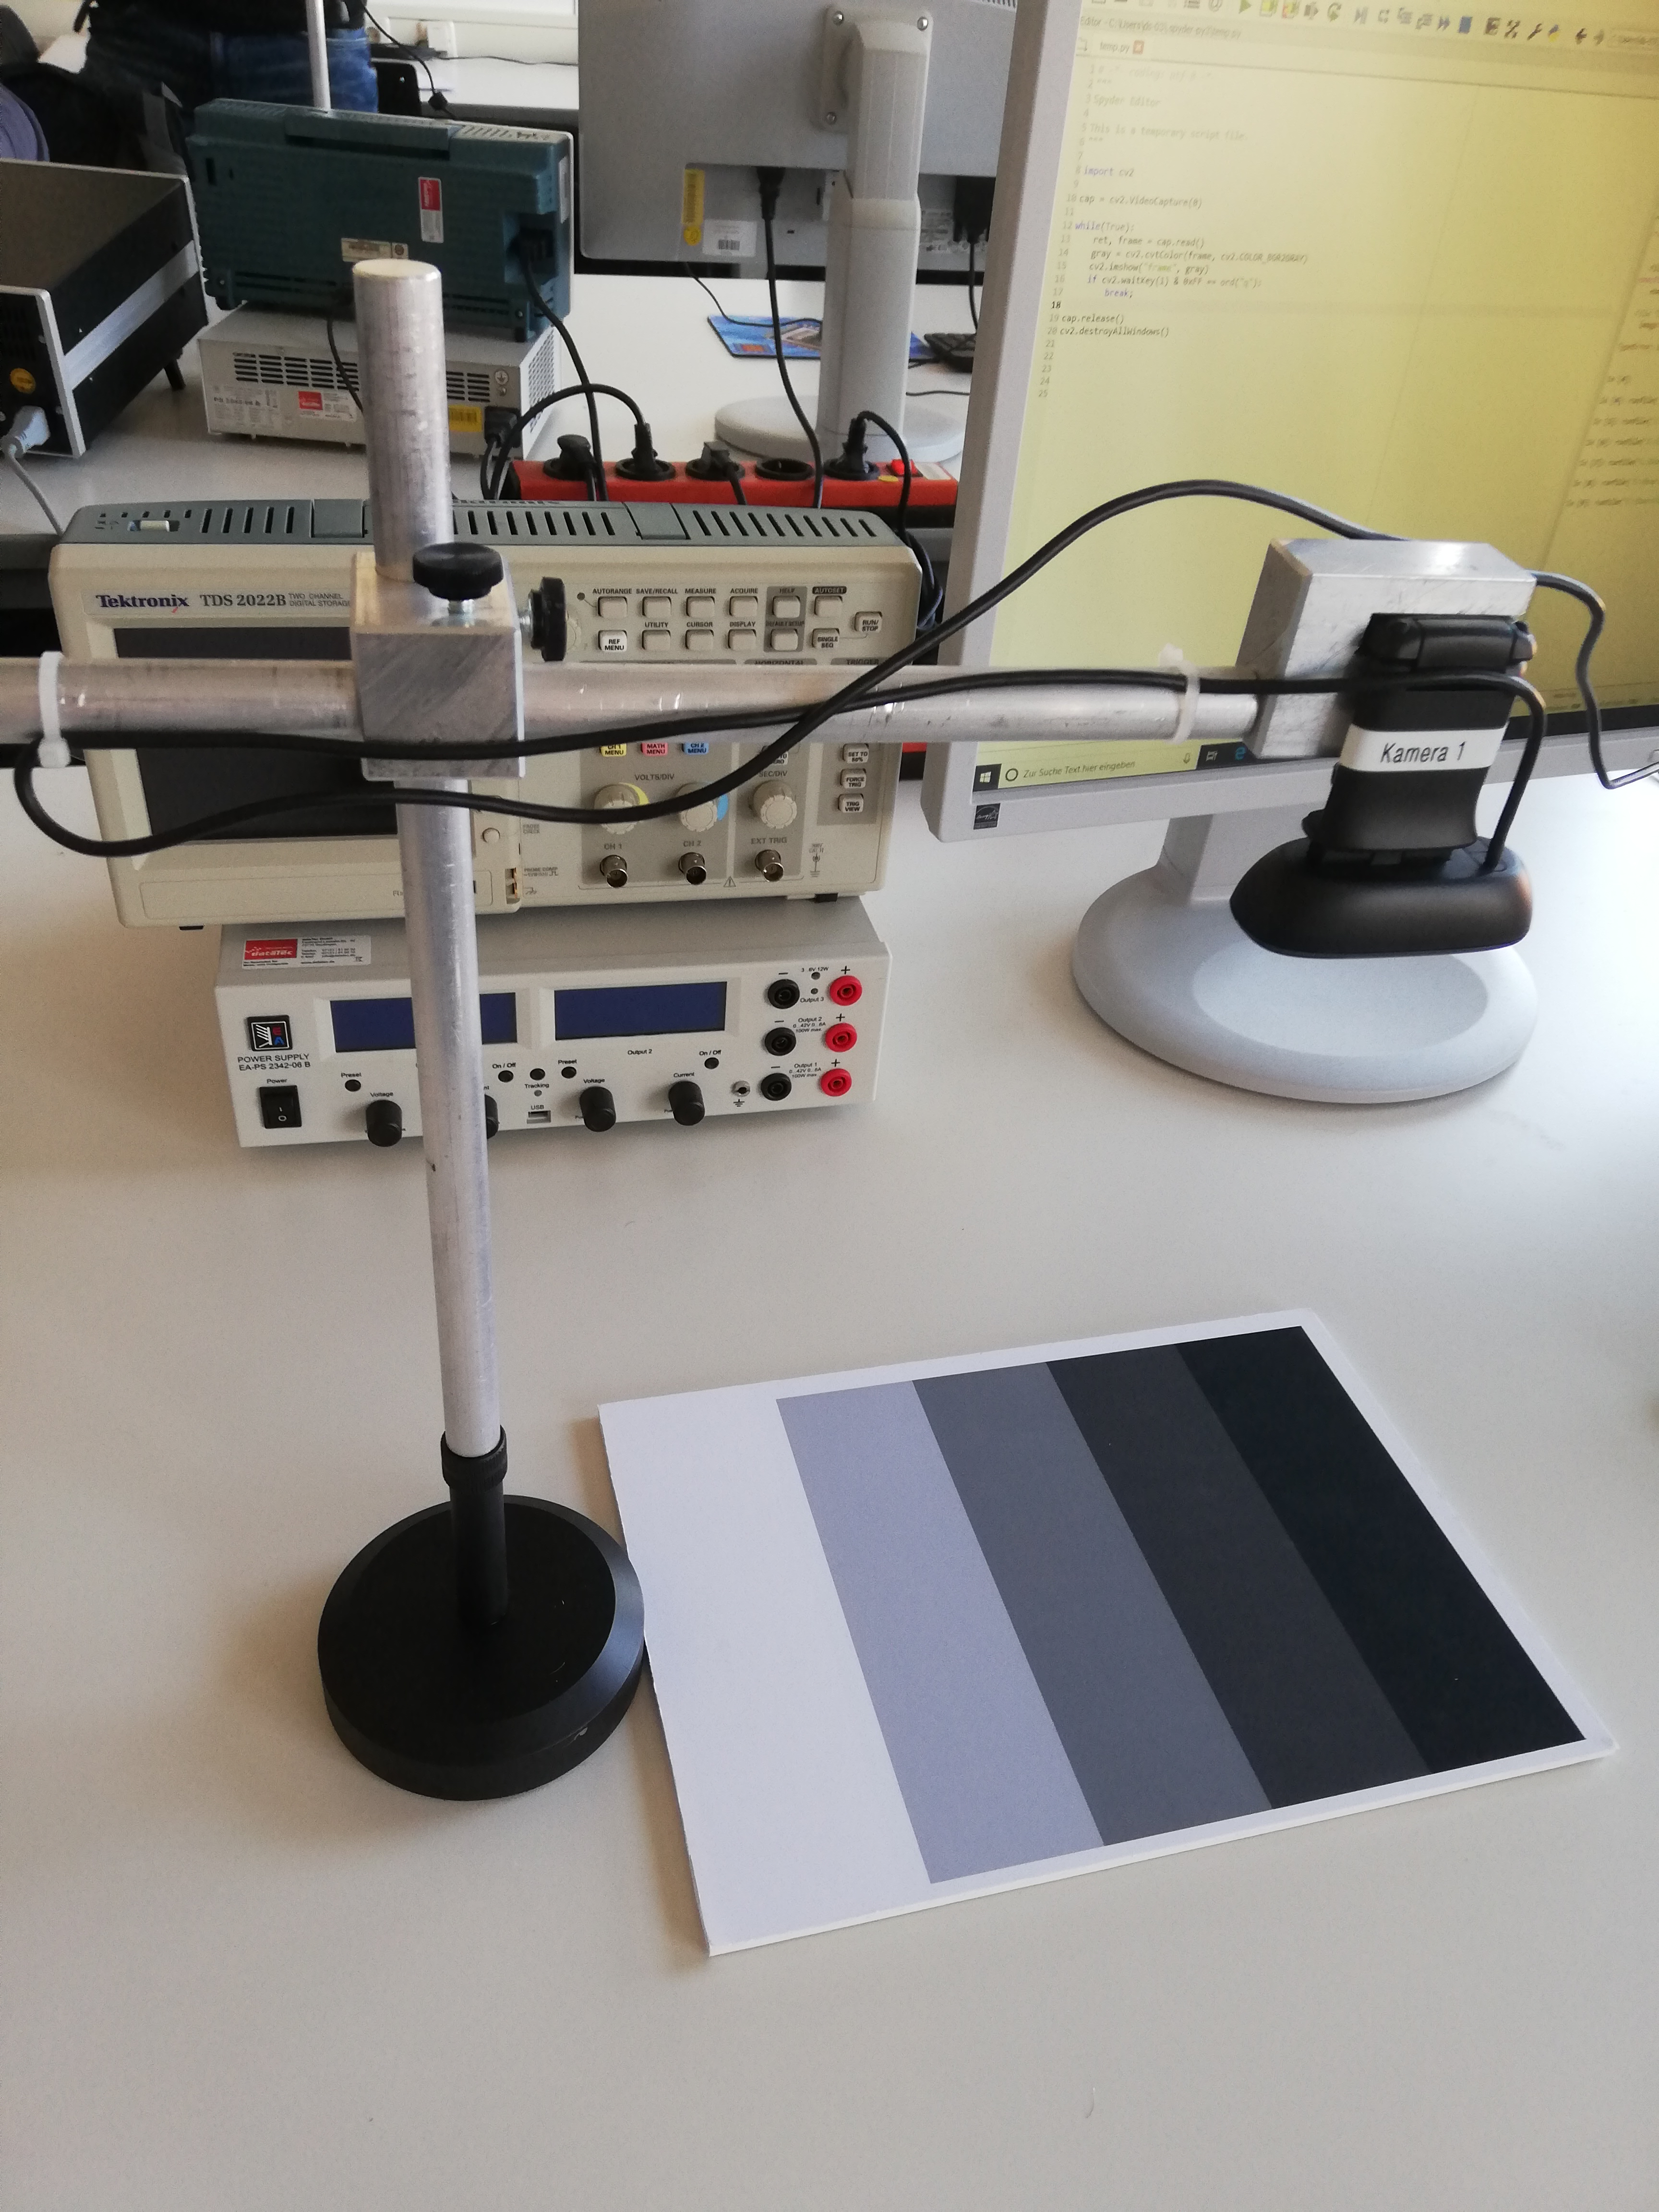
\includegraphics[width=0.7\textwidth]{media/aufbau.jpg}
	\caption{Aufbau im Labor}
	\label{fig:Aufbau im Labor}
\end{figure}
\newpage
\section{Messwerte}
\label{chap:VERSUCH_1_MESSWERTE}
Tabelle [\ref{chap:VERSUCH_1_MESSWERTE}] zeigt die von Hand notierten, sowie die in Python programmierten Werte.

\begin{table}[H]
	\centering\small
	\begin{tabular}{|c|c|c|c|c|c|}
		\hline
		Stufe & Blau, Rot und Grün & Hex-Value & Standartabweichung \\
		\hline
		Stufe 1 & 86.39761904761905 &  \#161616 & 2.082341260388545 \\
		\hline
		Stufe 2 & 112.00498456790123 &  \#1d1d1d & 2.6116529874626044 \\
		\hline
		Stufe 3 & 161.2048205596107 &  \#292929 & 2.2861194924984116 \\
		\hline
		Stufe 4 & 199.60105744949496 &  \#333333 & 2.968662423351764 \\
		\hline
		Stufe 5 & 235.58106563421828 &  \#3c3c3c & 2.582844019720398 \\
		\hline
	\end{tabular}
	\caption{Messwerte Kalibrierung}
	\label{fig:VERSUCH_1_MESSWERTE_TABELLE}
\end{table}

\newpage
\section{Auswertung}
\label{chap:VERSUCH_1_AUSWERTUNG}
In der folgenden Abbildung sind die Messergebnisse der durchschnittlichen Spannung nochmals visuell dargestellt. Die Messergebnisse wurden mit matplotlib in Python visualisiert.

Zuerst wurden die Werte von der .csv Datei mit \textit{genfromtxt()} in das Programm eingelesen.
Nachdem für die einzelnen Dateien mit der numpy Funktion \textit{np.mean()} der Durchschnitt der von dem Oszilloskop gemessen Ausgangsspannung in Volt ausgerechnet wurde, haben wir diese mit der y-Achse initialisiert.

Die x-Achse wurde mit dem Abstand in cm definiert. Durch eine For-Schleife kann nun jedem Abstandswert eine durchschnittliche Spannung zugewiesen werden.
\begin{figure}[H]
	\centering\small
	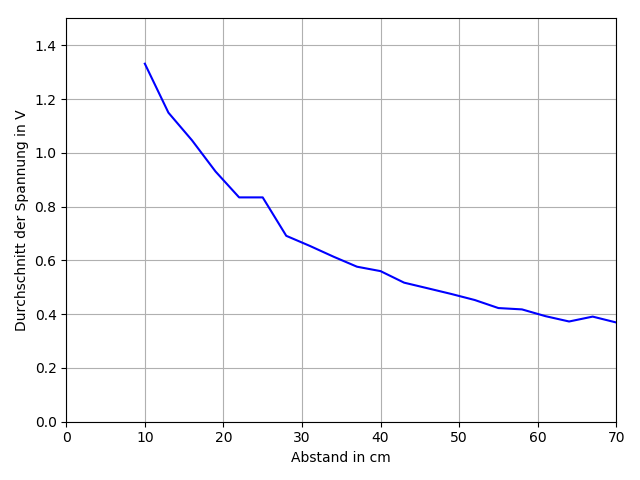
\includegraphics[width=\textwidth]{media/myplot.png}
	\caption{Durchschnittliche Spannung}
	\label{fig:VERSUCH_1_PLOT_DURCHSCNITTLICHE_SAPNNUNG}
\end{figure}

\newpage
In der folgenden Abbildung sind die Messergebnisse der Standardabweichung visuell dargestellt. Die Messergebnisse wurden mit matplotlib in Python visualisiert.
Hierfür wurde mit der numpy Funktion \textit{np.std()} die Standardabweichung in Volt berechnet und mit der y-Achse initialisiert.

Die x-Achse wurde wieder mit dem Abstand in cm deklariert. Wieder wurden durch die For-Schleife jedem Abstand ein Standardabweichung der Spannung zugewiesen werden.

\begin{figure}[H]
	\centering\small
	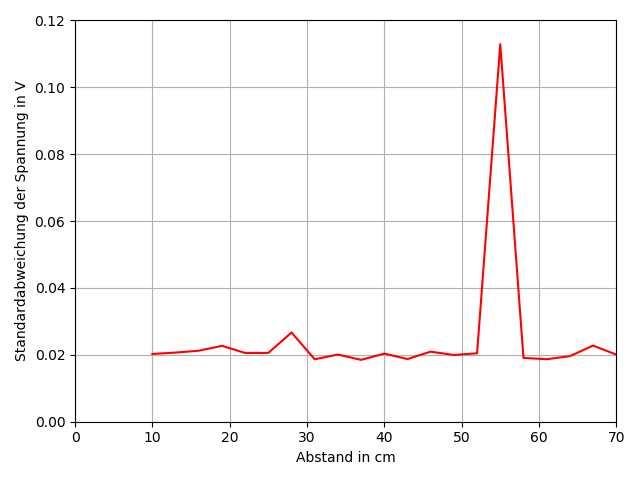
\includegraphics[width=\textwidth]{media/myplot2.png}
	\caption{Standartabweichung der Spannung}
	\label{fig:VERSUCH_1_PLOT_STANDARTABWEICHUNG}
\end{figure}

\newpage
\section{Interpretation}
\label{chap:VERSUCH_1_INTERPRETATION}
Wie man gut in der Tabelle und der Abbildung 2.2 ablesen kann, wird die Spannung stets niedriger. Dies liegt an der Anti-proportionalität, dass mit der zunehmenden Entfernung zwischen Holzbrett und Abstandssensor die vom Signalprozessor übertragene Spannung geringer wird. 
\newline
Leider haben wir bei der Generierung der Dateien einen Fehler gemacht und bei 22cm und 25cm zu spät die Single Sequenz aktualisiert, weshalb eine Gerade in dem Plot zwischen 22cm und 25cm genau gleich ist.
Zudem geht bei Messung zwischen 64cm und 67cm Abstand die Spannung nach oben. An dem Tag der Messung war das Wetter sehr wechselhaft, was zu einer Erhöhung der Werte führen könnte.
\newline
\newline
Bei der Messung 55cm ist eine sehr hohe Standardabweichung im Vergleich zu den anderen Werten. Dies liegt daran, dass das Oszilloskop durch andere Störfaktoren gestört wurde und so eine ungleiche Single Sequenz ergeben hat.
In dem rechten Bild der Abbildung 2.4 ist im Vergleich nochmals gut zu sehen, wie die hohe Standartabweichung zu stande kommt.

\begin{figure}[hbt!]
  	\centering
  	\subfloat[Messung bei 52cm]{
		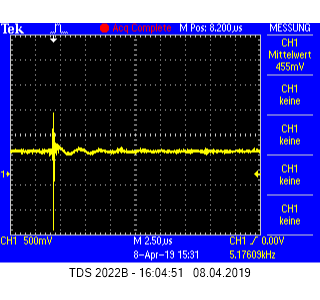
\includegraphics[width=0.4\textwidth]{media/52.png}\label{fig:f1}}
  	\hfill
  	\subfloat[Messung bei 55cm]{
		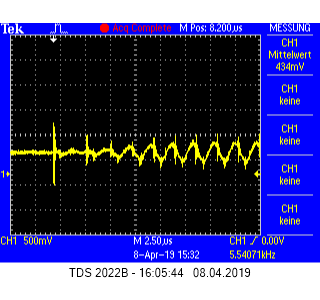
\includegraphics[width=0.4\textwidth]{media/55.png}\label{fig:f2}}
	\caption{Unterschiede durch Störfaktoren}
\end{figure}

%
% CHAPTER Versuch 2
%
\chapter{Versuch 2: Modellierung der Kennlinie durch lineare Regression}
\label{chap:VERSUCH_2}

\section{Fragestellung, Messprinzip, Aufbau, Messmittel}
\label{chap:VERSUCH_2_FRAGESTELLUNG}
In Versuch Nummer 2 war es die Aufgabe die Ein- und Ausgangswerte, also die Distanz und die durchschnittliche Spannung in der Tabelle zu logarithmieren.
\newline
Zudem soll man so eine Kennlinie, logarithmierte Werte sowie die lineare Regression darstellen.
\newline
So soll man die bereits erlernten Formeln aus den Vorlesungen in System, Signale und Sensoren anwenden und für die Daten des Sharp-Sensors umwandeln um so die Prinzipien der linearen Regression praktisch zu verwenden.
\newline
Durch die Errechnung und Darstellung der Kennlinie, soll man auch prüfen ob ein systematischer Fehler geschehen ist. Falls dies nicht der Falls ist, sollte die Kennlinie einer typischen Kennliniensteigung entsprechen.
\newline
Für den Versuch benötigt man lediglich die bereits gemessenen Daten, eine Python IDE, sowie die nützlichen Formeln aus den Vorlesungs- und Aufgabenblättern.
\newpage
\section{Messwerte}
\label{chap:VERSUCH_2_MESSWERTE}
Tabelle [\ref{chap:VERSUCH_2_MESSWERTE}] zeigt die in Python logarithmierten Werte.
\begin{table}[H]
	\centering\small
	\begin{tabular}{|c|c|c|}
		\hline
		Distanz & log cm & log Durchschnitt \\
		\hline
		10cm & 2.302585092994046 & 0.28658251236288684 \\
		\hline
		13cm & 2.5649493574615367 & 0.13950997769809692 \\
		\hline
		16cm & 2.772588722239781 & 0.04584587706574458 \\
		\hline
		19cm & 2.9444389791664403 & -0.0717653956802384 \\
		\hline
		22cm & 3.091042453358316 & -0.18091598142798918 \\
		\hline
		25cm & 3.2188758248682006 & -0.18091598142798918 \\
		\hline
		28cm & 3.332204510175204 & -0.3688220785875914 \\
		\hline
		31cm & 3.4339872044851463 & -0.42460823943365683 \\
		\hline
		34cm & 3.5263605246161616 & -0.48755538925392977 \\
		\hline
		37cm & 3.6109179126442243 & -0.5504620343701235 \\
		\hline
		40cm & 3.6888794541139363 & -0.579426134298413 \\
		\hline
		43cm & 3.7612001156935624 & -0.659127119920277 \\
		\hline
		46cm & 3.828641396489095 & -0.7003660010868976 \\
		\hline
		49cm & 3.8918202981106265 & -0.7438412790564594 \\
		\hline
		52cm & 3.9512437185814275 & -0.792597814482305 \\
		\hline
		55cm & 4.007333185232471 & -0.8607681589957209 \\
		\hline
		58cm & 4.060443010546419 & -0.8726037472131969 \\
		\hline
		61cm & 4.110873864173311 & -0.9348943146021321 \\
		\hline
		64cm & 4.1588830833596715 & -0.9865867500420398 \\
		\hline
		67cm & 4.204692619390966 & -0.9389225676676274 \\
		\hline
		70cm & 4.248495242049359 & -0.9965499402651674 \\
		\hline
	\end{tabular}
	\caption{Logarithmus von der Distanz und der Durchschnittsspannung}
	\label{fig:VERSUCH_2_LOGARITHMUS_TABELLE}
\end{table}
\newpage
\section{Auswertung}
\label{chap:VERSUCH_2_AUSWERTUNG}
In der folgenden Abbildung wurden die Messergebnisse logarithmiert und daraufhin mit matplotlib in Python visualisiert.
Die Werte wurden mit der Funktion \textit{genfromtxt()} aus der .csv Datei in das Programm eingelesen.
Die Distanz in cm wurde mit der numpy Funktion \textit{np.log()} logarithmiert. Die durchschnittlichen Spannung in Volt wurde ebenfalls mit \textit{np.log(np.mean())} logarithmiert. 
Während die x-Achse mit dem logarithmierten Wert von dem Abstand belegt wird, initialisiert man die y-Achse mit dem logarithmierten Durchschnitt der Spannung in Volt.

\begin{figure}[hbt!]
	\centering\small
	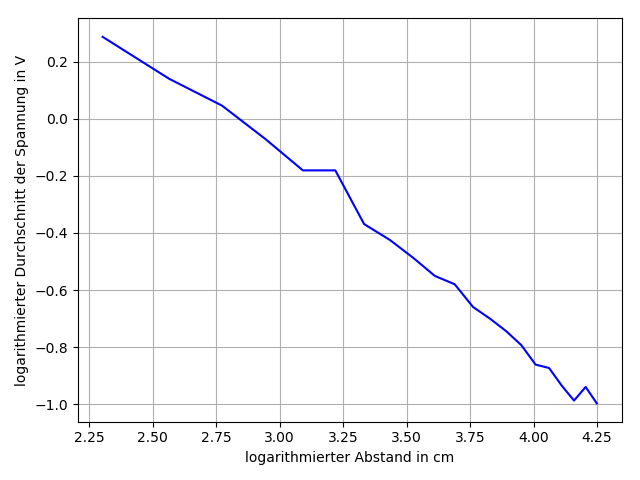
\includegraphics[width=\textwidth]{media/myplot4.png}
	\caption{Logarithmus der Ein- und Ausgangswerte}
	\label{fig:Logarithmus der Ein- und Ausgangswerter}
\end{figure}
\newpage
In der folgenden Abbildung wurde die Kennlinie visualisiert mit matplotlib in Python.
\newline
Da die Werte bereits eingelesen wurden in der vorherigen Darstellung müssen wir dies nicht erneut machen.
Hier werden erneut die logarithmierten Abstände in cm verwendet, sowie der logarithmierte Durchschnitt der Spannung in Volt. Ebenfalls brauchen wir die Steigung.
Wir benötigen die folgende Formel, welche auf dem Aufgabenblatt auf Seite 3 vorzufinden ist:
\textit{y\textsuperscript{'} = ln y = ln(x\textsuperscript{a}) = a * ln(x) = a * ln(e\textsuperscript{x\textsuperscript{'}}) = a * x\textsuperscript{'}}
\newline
\newline

\begin{figure}[hbt!]
	\centering\small
	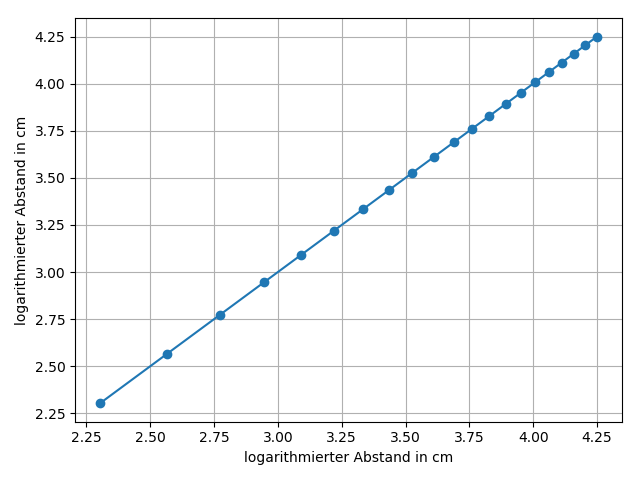
\includegraphics[width=\textwidth]{media/myplot5.png}
	\caption{Kennlinie}
	\label{fig:Kennlinie}
\end{figure}
\newpage
In der folgenden Abbildung wurde die Lineare Regression realisiert mit matplotlib in Python.
Auch hier wurden die Werte die Werte bereits eingelesen, weshalb dieser Schritt entfällt.
\newline
Hier werden erneut die logarithmierten Abstände in cm verwendet, sowie der logarithmierte Durchschnitt der Spannung in Volt. 
Sämtliche logarithmierten Abstände in cm wurden in ein Array gemacht, was später für die x-Achse verwendet wird.
Die Werte für die logarithmierten Durchschnitte der Spannung in Volt wurden ebenfalls in ein seperates Array gepackt, welche später wiederrum für die y-Achse verwendet werden.
\newline
\newline
Danach wurde stats.lingress() in folgender Darstellung verwendet:
\newline
\textit{gradient, intercept, r\_value, p\_value, std\_err = stats.linregress(x, y)}
\newline
Danach wird noch die folgende Formel angewendet: 
\textit{y\textsuperscript{'} = a *  x\textsuperscript{'} + b}
\newline
In Python sieht diese Formel folgendermaßen aus: \textit{y1 = gradient * x1 + intercept} \& \textit{x1 = np.linspace(mn, mx, 500)}
\textit{y1} wird mit \textit{x1} als Ausgleichsgerade der linearen Regression angezeigt.
x und y wurden bereits vorher in ein Array gespeichert und nun als Punkte angezeigt.
\newline
Die Ausgleichsgerade macht den Abstand zu den Punkten im Gesamten minimal.
\begin{figure}[hbt!]
	\centering\small
	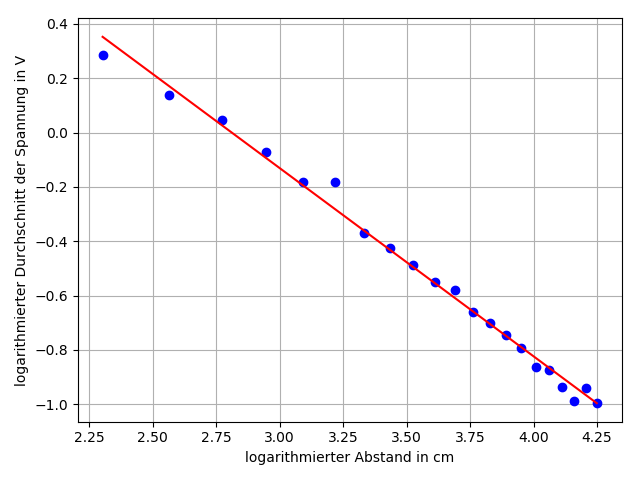
\includegraphics[width=0.9\textwidth]{media/myplot3.png}
	\caption{Lineare Regression}
	\label{fig:Lineare Regression}
\end{figure}
\newpage
\section{Interpretation}
\label{chap:VERSUCH_2_INTERPRETATION}
In Abbildung 3.1 sieht man nur wenige Unstimmigkeiten.
Bei der x-Achse an der Stelle 3.25cm liegt der Fehler an der Messung, für die unsere Messung verantwortlich ist.
Leider haben wir denselben Wert zweimal eingelesen, ohne die Single Sequenz zu aktualisieren, was zu diesem Ausschlag führt.

Kurz vor dem Ende der Visualisierung geht der Wert nach oben, was an einer Erhöhung der Spannung liegt. Dies ist auch sichtbar in der Tabelle 2.1.
Vermutlich ist dies passiert durch veränderte Wetterverhältnisse, die die Lichtverhältnisse im Raum veränderten.
\newline
\newline
Die Kennlinie in Abbildung 3.2 weißt auch keine systematischen Fehler auf, da sie einer Kennliniensteigung beziehungsweise der Sensitivät eines Sensors entspricht.

Das heißt, dass bei einem doppelten Eingangswert auch der doppelte Ausgangswert ausgegeben wird.
\newline
\newline
In Abbildung 3.3 zieht sich die Ausgleichsgerade durch die einzelnen Punkte um den Abstand minimal werden zu lassen. Abgesehen von einzelnen Ausreißern wie zum Beispiel dem Wert bei 3.25cm, der durch einen Messfehler entstanden ist wie schon weiter oben berichtet, liegen die Punkte sehr nah an der Ausgleichsgeraden.

Dies lässt darauf deuten, dass die meisten Punkte durch den Abstandssensor richtig gemessen wurden.
%
% CHAPTER Versuch 3
%
\chapter{Versuch 3: Flächenmessung mit Fehlerrechnung}
\label{chap:VERSUCH_3}

\section{Fragestellung, Messprinzip, Aufbau, Messmittel}
\label{chap:VERSUCH_3_FRAGESTELLUNG}
Im dritten Versuch ist eine Aufgabe die Ermittlung des Messfehlers des Abstandsmessers. Zuerst müssen wir die lange Seite eines DinA4 Blattes vom Sensor müssen und danach das Resultat als  .csv Datei speichern. 
\newline
So müssen wir zur Ermittlung des Messfehlers die Fehlerfortpflanzung durch die folgende Kennlinie berechnen: 
\newline
\textit{e\textsuperscript{b} *  x\textsuperscript{a}}
Zudem muss man berechnen wie groß der Vertrauensbereich für eine Sicherheit von 68\% und für eine Sicherheit von 95\% berechnen. Danach sollten wir die Fehlerfortpflanzung dazu benutzen um das Ergebnis der Abstandsmessung in cm angeben zu können.
\newline
\newline
Im zweiten Teil des dritten Versuchs müssen wir nun die breite Seite eines DinA4 Blattes messen. Daraufhin sollen wir mit der selben Methode die Breite des Blattes berechnen und die Fläche des Blattes berechnen. Dies geschieht mithilfe dem Gaußschen Fehlerfortpflanzungsgesetz.
\newpage
\section{Messwerte}
\label{chap:VERSUCH_3_MESSWERTE}
Tabelle [\ref{chap:VERSUCH_3_MESSWERTE}] zeigt die durchschnittliche Spannung in Volt für die breite und die lange Seite eines DinA4 Blattes.
\begin{table}[H]
	\centering\small
	\begin{tabular}{|c|c|}
		\hline
		Distanz &  durchschnittliche Spannung in Volt \\
		\hline
		29,7cm & 0.6583416425026114V \\
		\hline
		21cm & 0.8572027683256641V \\
		\hline
	\end{tabular}
	\caption{Messwerte DinA4}
	\label{fig:VERSUCH_3_MESSWERTE_DINA4}
\end{table}
\section{Auswertung}
\label{chap:VERSUCH_3_AUSWERTUNG}
Tabelle [\ref{chap:VERSUCH_3_MESSWERTE}] zeigt die berechneten Messfehler im Vertrauensbereich bei einer Distanz von 29,7cm.
Für die Berechnung des Messfehlers bei den entsprechenden Vertrauensbereichen der Gaußverteilung benötigt man die folgende Formel:
\newline
\textit{x = Durchschnitt der Spannung in Volt + Korrekturfaktor * Standardabweichung + (2sx oder 4sx, je nach Vertrauensbereich)}
\newline 
\newline 
In Python wird die Formel folgendermaßen ausgeführt:
\newline 
\textit{result1 = np.mean(data2) + 1,95 * (np.std(data2) / np.sqrt(1000)) * 4}
Der Vertrauensbereich bei 68\% hat einen Korrekturfaktor von 1 und  ist +-1sx groß  , während der der Vetrauensbereich bei 95\% einen Korrekturfaktor von 1,96 hat und +-2sx groß ist.
\newline 
\textit{np.mean} ist hier eine numpy Funktion welche den Durchschnitt berechnet, wie hier die durchschnittliche Spannung in Volt für die lange Seite der DinA4 Seite.
\newline 
\newline 
\textit{np.std} ist ebenfalls eine numpy Funktion und berechnet die Standardabweichung in cm für die lange Seite der DinA4 Seite.
\newline 
\textit
Diese wird durch die numpy Funktion { np.sqrt(1000)} ist ebenfalls eine numpy Funktion und berechnet die Wurzel. In diesem Fall soll die Funktion die Anzahl der verwendeten Spannungen pro Messung die Wurzel ziehen. 
\begin{table}[H]
	\centering\small
	\begin{tabular}{|c|c|}
		\hline
		 Formel &  Ergebnis \\
		\hline
		68\% = 0.6583416425026114V + 1 * 0.0006520905314570869V * 2sx & 0.6596458235655256cm \\
		\hline
		95\% = 0.6583416425026114V + 1,96 * 0.0006520905314570869V * 4sx & 0.6634540322692349cm \\
		\hline
	\end{tabular}
	\caption{Messfehler in Gaußverteilung}
	\label{fig:VERSUCH_3_MESSFEHLER_TABELLE}
\end{table}

Tabelle [\ref{chap:VERSUCH_3_MESSWERTE}] zeigt die Ergebnisse der Abstandsmessung mittels der Fehlerfortpflanzung an.
Verglichen werden die Gaußverteilungen von 68\% und 95\% mit den Distanzen eines DinA4 Blattes.
Um diese Formel zu berechnen benötigen wir noch \textit{a} und \textit{b}. 
\newline \textit{a} erhält man durch den Logarithmus aus der Länge bzw. der Breite des Blattes geteilt durch die Logarithmierung der durchschnittlichen Spannung:
\newline 
\textit{a1 = np.log(29.7) / np.log(np.mean(data2))}
\newline
\newline
\textit{b} wiederrum erhält man aus dem Logarithmus der Distanz subtrahiert von der Multiplikation von dem Logarithmus der durchschnittlichen Spannung in Volt und a:
\newline
\textit{b1 = np.log(29.7) - (a1 * np.log(np.mean(data2)))}
\newline
Um die Abstandsmessung mit der Fehlerfortpflanzung zu berechnen benötigt man zuerst die folgende Formel:
\newline 
\textit{e\textsuperscript{b} *  x\textsuperscript{a}}.
\newline 
Bzw. deren Ableitung:
\textit{e\textsuperscript{b} * a * x\textsuperscript{a-1}}. Nun nur noch  die errechneten Werte einfügen.
\newline 
\newline 
Wenn man ein Vertrauensintervall von 68\% verwendet, muss man nur noch die abgeleitete Funktion mit der Standardabweichung geteilt durch die Wurzel mit der Anzahl der Messungen multiplizieren und schon hat man den Vertrauensintervall.
Für den Vertrauensintervall von 95\% hingegen muss man noch zusätzlich den Vertrauensfaktor von 1,96 mulitplizieren.
\newline 
\begin{table}[H]
	\centering\small
	\begin{tabular}{|c|c|c|}
		\hline
		Sicherheit & Distanz &  Abstandsmessung \\
		\hline
		68\% & 21cm & 0.31835908731736245cm \\
		\hline
		68\% & 29,7cm & 0.23864419265666054cm \\
		\hline
		95\% & 21cm & 0.6239838111420121cm \\
		\hline
		95\%  & 29,7cm & 0.4677426176070423cm \\
		\hline
	\end{tabular}
	\caption{Abstandsmessung mit Fehlerfortpflanzung}
	\label{fig:VERSUCH_3_FEHLERFORTPFLANZUNG_ABSTANDSMESSUNG_TABELLE}
\end{table}
\newpage
Wenn man die Länge und die Breite eines DinA4 Blattes multipliziert, erhält man den 
\newline
Flächeninhalt. 
\newline
29,7cm Länge * 21cm Breite = 623,7cm\textsuperscript{2}.
\newline
Damit hat ein DinA4 Blatt einen Flächeninhalt von 623.7 cm\textsuperscript{2}.
\newline
\newline
Um den Messfehler in einem Vertrauensbereich von 68\% mit 623.7cm\textsuperscript{2} Flächeninhalt zu berechnen muss man nur die Werte von 68\% addieren: 
\newline
0.557003279974023cm.
\newline
Um den Messfehler in einem Vertrauensbereich von 95\% hat mit 623.7cm\textsuperscript{2}zu berechnen muss man nur die Werte von 95\% addieren: 
\newline
1.0917264287490545cm.
\section{Interpretation}
\label{chap:VERSUCH_3_INTERPRETATION}
Die Messfehler auf den Flächeninhalt eines DinA4 Blattes bezogen
\newline
\begin{table}[H]
	\centering\small
	\begin{tabular}{|c|c|}
		\hline
		Vertrauensintervall &  Messfehler \\
		\hline
		68\% & 0.557003279974023cm \\
		\hline
		95\%  & 1.0917264287490545cm \\
		\hline
	\end{tabular}
	\caption{Messfehler im Gaußsche Intervall}
	\label{fig:VERSUCH_3_FLACHENINHALT_VERTRAUENSINTERVALL}
\end{table}
Die Höhe der Messunsicherheit hängt mit der Anzahl der Messungen zusammen: Zum Beispiel bei einem Vertrauensintervall von 95\%, aber nur 2 Messungen gibt es einen Korrekturfaktor von 12,71.
\newline
Zudem gilt: Desto höher der Vertrauensintervall, desto höher sind auch die Werte.
Dies trifft hier, als auch in Tabelle 4.3 zu, da die Messunsicherheit hier bei 95\% doppelt so hoch ist, wie die bei 68\%.
\newline
Diese erhöhten Werte kommen durch einen erhöhten Korrekturfaktor.

\newline

%
% CHAPTER Anhang
%
\renewcommand\thesection{A.\arabic{section}}
\renewcommand\thesubsection{\thesection.\arabic{subsection}}

\chapter*{Anhang}
\label{chap:APPENDIX}
\addcontentsline{toc}{chapter}{Anhang}
%\setcounter{chapter}{0}
\addtocounter{chapter}{1}
\setcounter{section}{0}

\section{Quellcode}
\label{chap:APPENDIX_SOURCECODE}

\subsection{Quellcode Versuch 1: Messung Kalibrierung}
\label{chap:APPENDIX_SOURCECODE_V1}
\lstinputlisting[style=PYTHON, frame=single, caption=Ermittlung der Kennlinie des Abstandssensors, captionpos=b, label=lst:APPENDIX_SOURCECODE_MEASURE]{../task1.1.py}
\lstinputlisting[style=PYTHON, frame=single, caption=Ermittlung der Kennlinie des Abstandssensors, captionpos=b, label=lst:APPENDIX_SOURCECODE_MEASURE]{../task1.2.py}
\lstinputlisting[style=PYTHON, frame=single, caption=Ermittlung der Kennlinie des Abstandssensors, captionpos=b, label=lst:APPENDIX_SOURCECODE_MEASURE]{../task1.3.py}
\newpage
\subsection{Quellcode Versuch 2}
\label{chap:APPENDIX_SOURCECODE_V2}
\lstinputlisting[style=PYTHON, frame=single, caption=Lineare Regression, captionpos=b, label=lst:APPENDIX_SOURCECODE_REGRESSION]{../task2.1.py}
\lstinputlisting[style=PYTHON, frame=single, caption=Lineare Regression, captionpos=b, label=lst:APPENDIX_SOURCECODE_REGRESSION]{../task2.2.py}
\newpage
\subsection{Quellcode Versuch 3}
\label{chap:APPENDIX_SOURCECODE_V3}
\lstinputlisting[style=PYTHON, frame=single, caption=Flächenmessung mit Fehlerrechnung, captionpos=b, label=lst:APPENDIX_SOURCECODE_AREA1]{../task3.1.py}
\lstinputlisting[style=PYTHON, frame=single, caption=Flächenmessung mit Fehlerrechnung, captionpos=b, label=lst:APPENDIX_SOURCECODE_AREA2]{../task3.2.py}
\lstinputlisting[style=PYTHON, frame=single, caption=Flächenmessung mit Fehlerrechnung, captionpos=b, label=lst:APPENDIX_SOURCECODE_AREA3]{../task3.3.py}
\lstinputlisting[style=PYTHON, frame=single, caption=Flächenmessung mit Fehlerrechnung, captionpos=b, label=lst:APPENDIX_SOURCECODE_AREA4]{../task3.4.py}
\lstinputlisting[style=PYTHON, frame=single, caption=Flächenmessung mit Fehlerrechnung, captionpos=b, label=lst:APPENDIX_SOURCECODE_AREA5]{../task3.4b.py}
\lstinputlisting[style=PYTHON, frame=single, caption=Flächenmessung mit Fehlerrechnung, captionpos=b, label=lst:APPENDIX_SOURCECODE_AREA5]{..dead.py}
\lstinputlisting[style=PYTHON, frame=single, caption=Flächenmessung mit Fehlerrechnung, captionpos=b, label=lst:APPENDIX_SOURCECODE_AREA5]{../dead2.py}
\newpage
\section{Messergebnisse}
\label{chap:APPENDIX_MEASUREMENT_SOURCE}
\begin{figure}[hbt!]
	\centering\small
	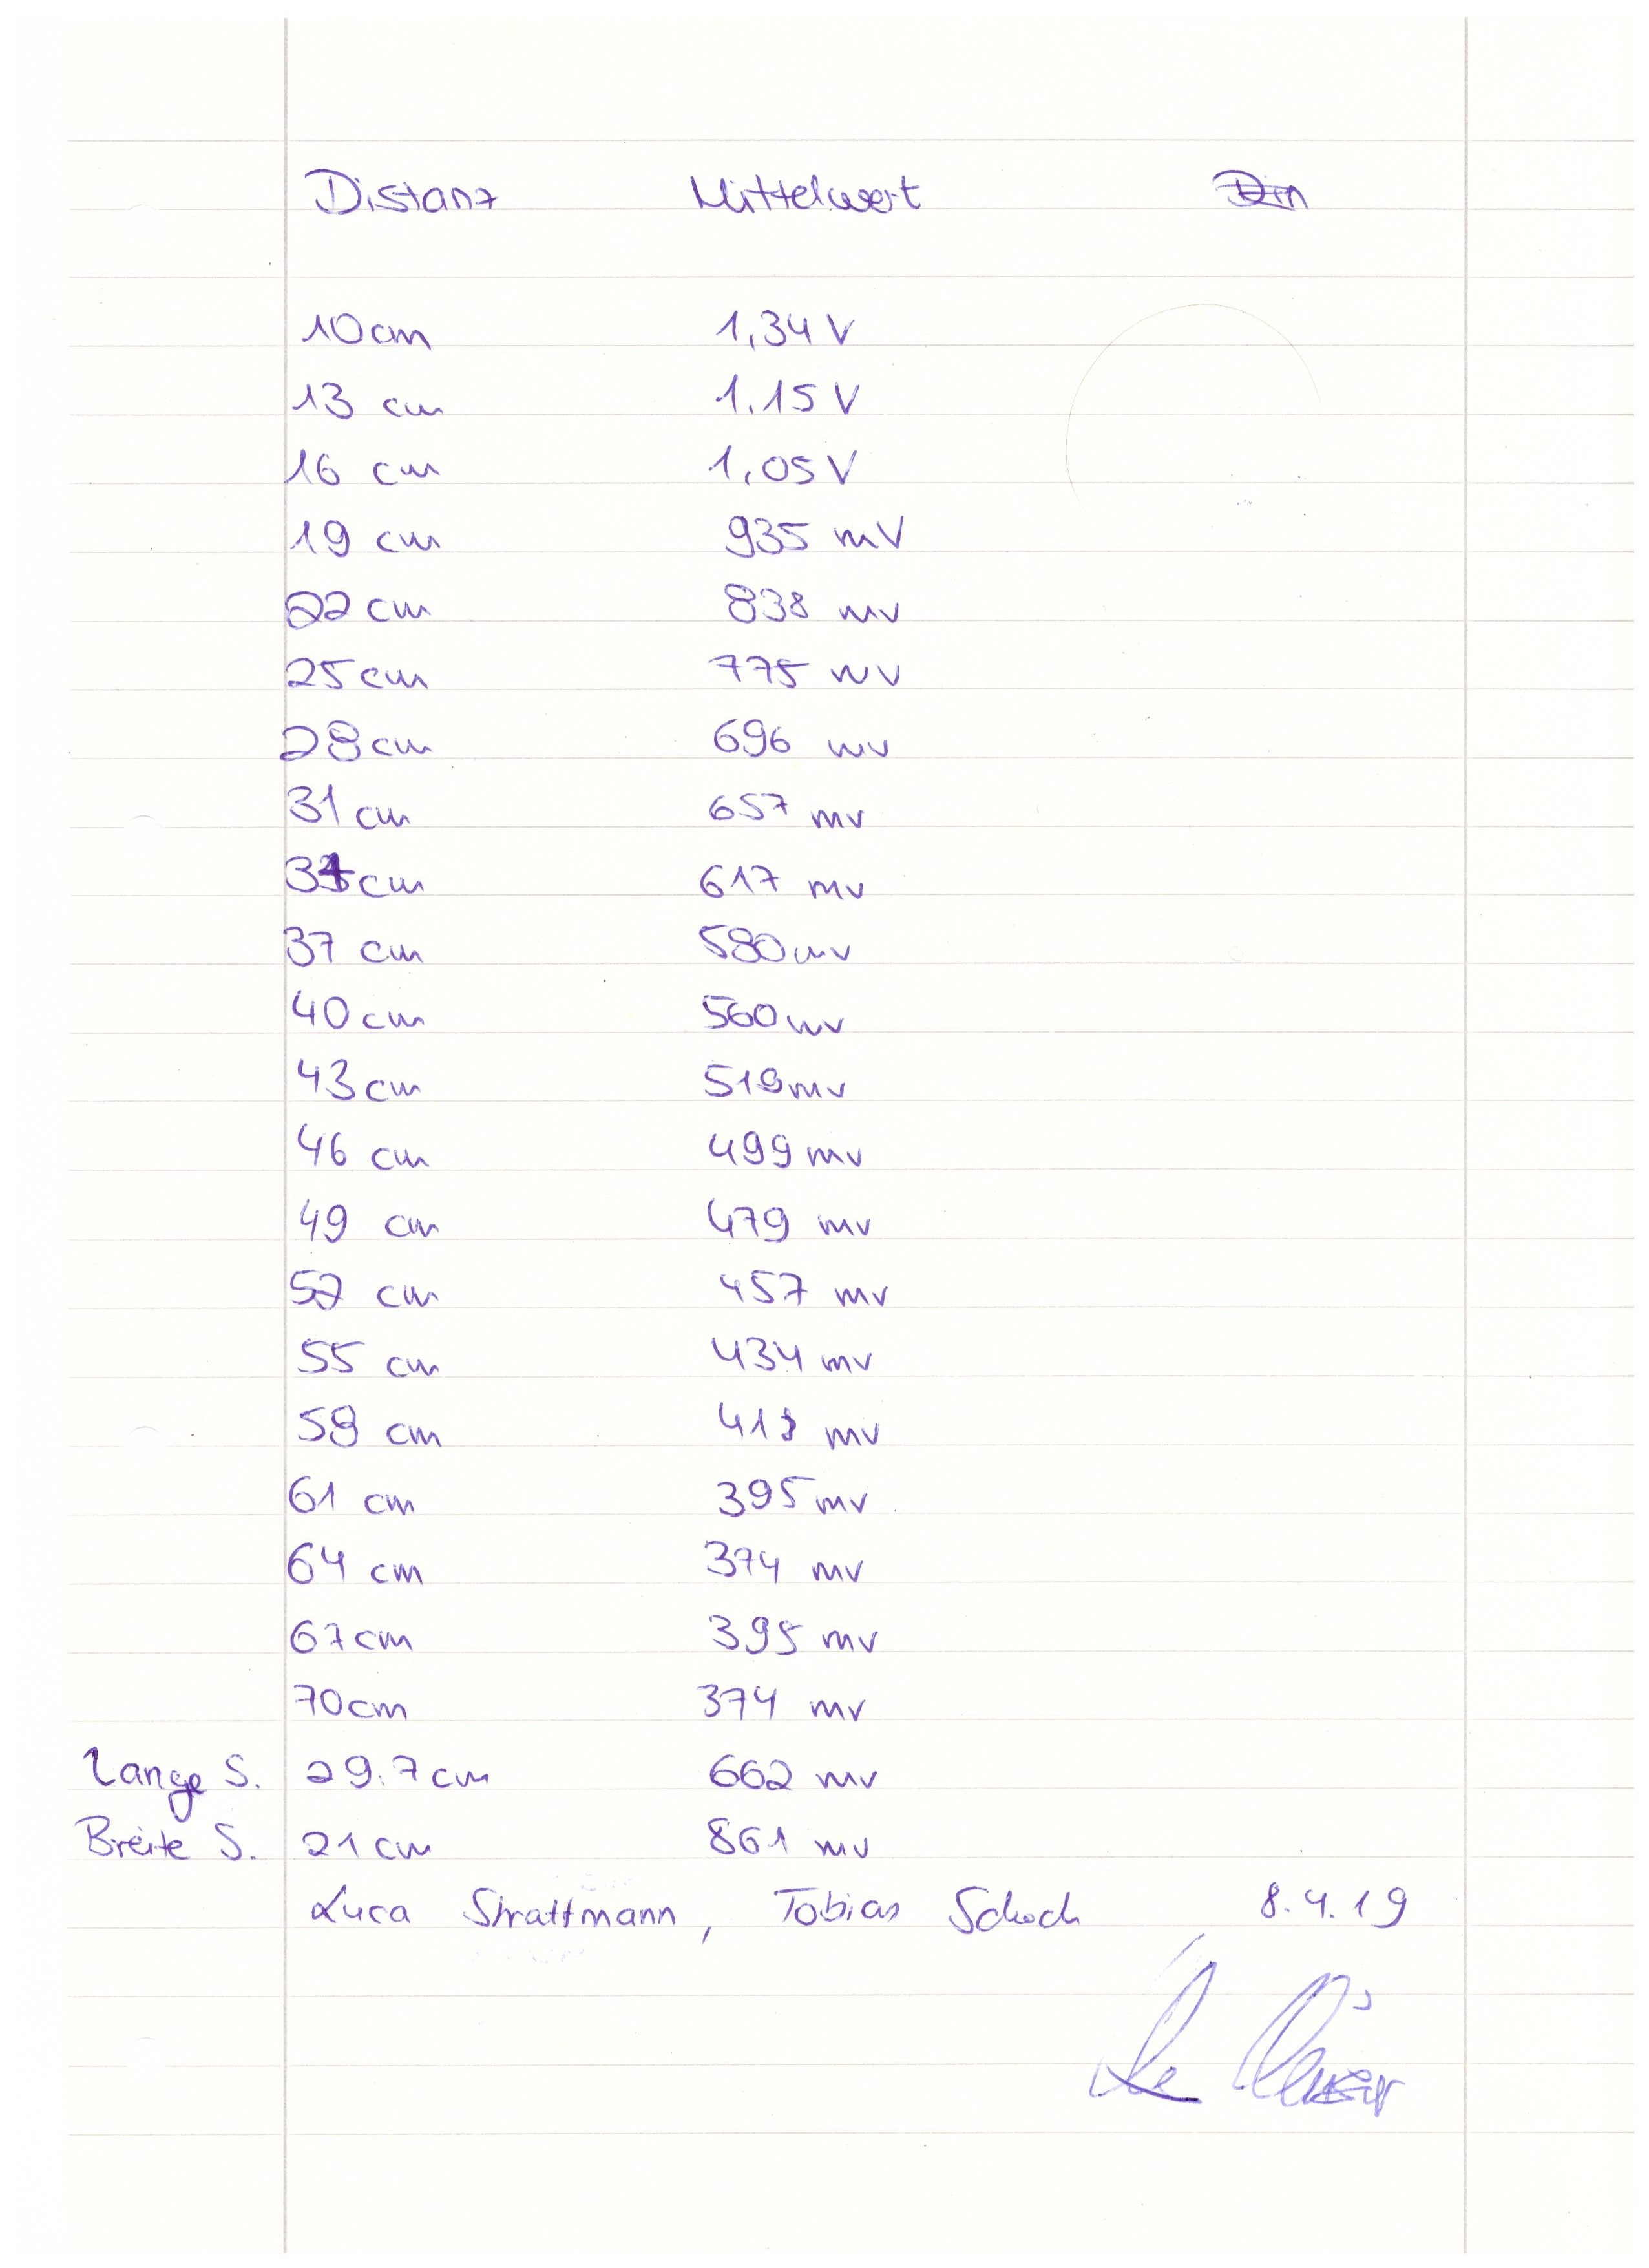
\includegraphics[width=0.8\textwidth]{media/scan.png}
	\caption{Messungen aus dem Labor}
	\label{fig:Messungen aus dem Labor}
\end{figure}

%
% Literaturverzeichnis
%
%\setcounter{chapter}{0}
\addtocounter{chapter}{1}
\setcounter{section}{1}

%
% Literaturverzeichnis
%
\phantomsection
\addcontentsline{toc}{chapter}{Literaturverzeichnis}
\bibliography{../references}
\newpage

\end{document}


\end{document}
%------------------------------------
% ╔═╗╔╗╔╔╦╗  ╔╦╗╔═╗╔═╗╦ ╦╔╦╗╔═╗╔╗╔╔╦╗
% ║╣ ║║║ ║║   ║║║ ║║  ║ ║║║║║╣ ║║║ ║ 
% ╚═╝╝╚╝═╩╝  ═╩╝╚═╝╚═╝╚═╝╩ ╩╚═╝╝╚╝ ╩ 
%------------------------------------